\chapter{Smart Cafeteria Design}
\label{chap:DesignofSmartCafeteria}
In this chapter, I have discussed the design of ``Smart Cafeteria''. In first
[\ref{sec:CAD}] and second [\ref{sec:SOA}] section, conceptual architecture and
design and service oriented architecture (SOA) was discussed respectively. These
are the top level architecture and design of the system. In the next section
[\ref{sec:PrototypeSC}] prototype of ``Smart Cafeteria'' is discussed; a mid
fidelity prototype of all functionalities of the system; some of them was
covered in desktop prototype [\ref{subsec:prototypefordesktop}] and the rest was
covered in mobile prototype [\ref{subsec:PrototypeforMobile}]. And the final
section [\ref{sec:keyFeaturesSC}] was discussed about the key features of the
system.

\section{Conceptual Architecture And Design}
\label{sec:CAD}
A conceptual architecture~\cite{Zamg} describes essential and top level features
of a system and identifies the main processes and their flows taking place in
the system. It provides a definition of the phenomenon in terms of features
recognizable by analysis and observations; and describes the abstract life cycle
of the system.

Conceptual design~\cite{MicrosoftCorporation2003} is the process of gathering,
analyzing, and prioritizing business and user perspectives of the problem and
the solution, and then creating a high-level representation of the solution.
Conceptual design should follow three principle steps in any system
development life cycle; research, analysis and optimization by system designer.


In the figure \ref{ConceptualArchitecture_top_level} a top level architecture of
``Smart Cafeteria'' application is shown.
The mobile appplication users interact with the system through interface of the
mobile application and desktop users interact with the system through browser.
\begin{figure}[h!t]
    \centering
      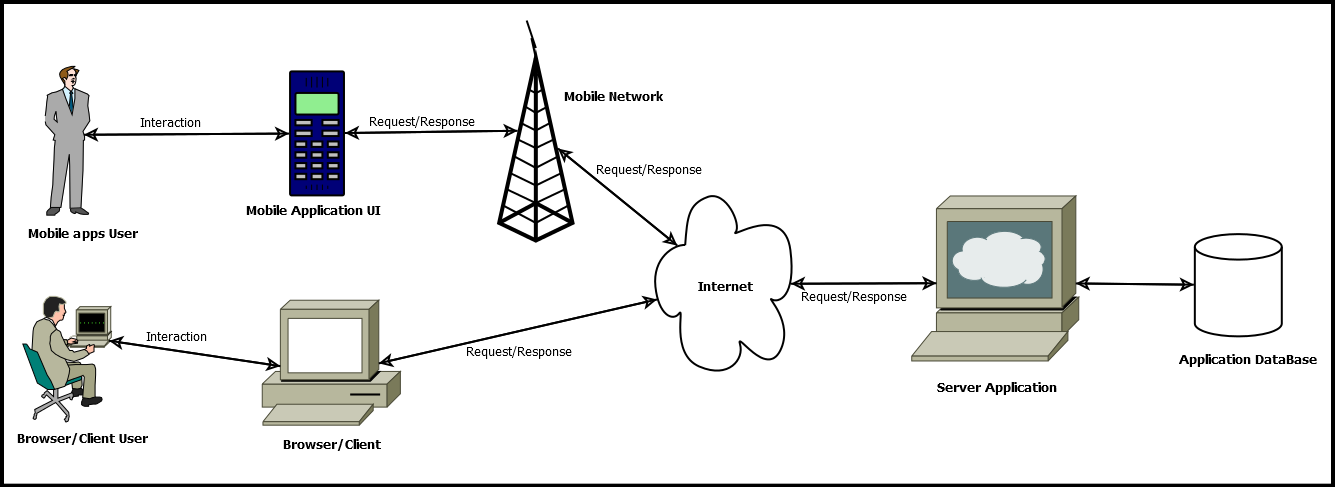
\includegraphics[width=5.5in]{ch4/SOA/ConceptualArchitecture}
  \caption{Conceptual Architecture of Smart Cafeteria[Top Level]}
  \label{ConceptualArchitecture_top_level}
\end{figure}

\begin{figure}[h!t]
    \centering
      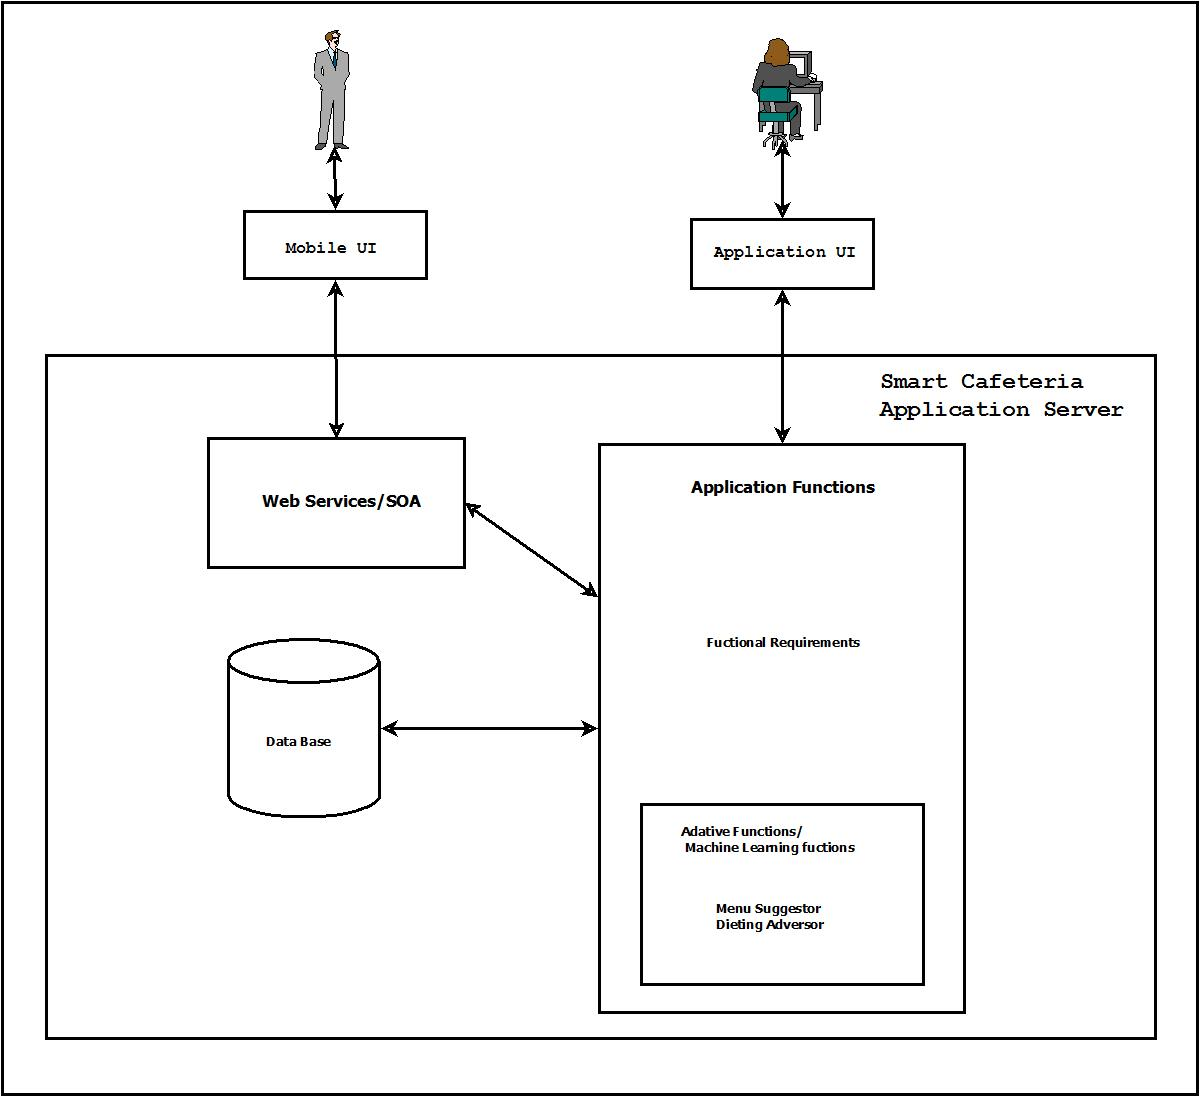
\includegraphics[width=5.5in,height=5in]{ch4/SOA/ConceptualArchitecture_new}
  \caption{Conceptual Design of Smart Cafeteria[Server Level]}
  \label{ConceptualArchitecture_server_level}
\end{figure}
In the figure~\ref{ConceptualArchitecture_server_level}, server level
conceptual design has been shown where application fuctionalities and
web services/SOA intergrates together to support mobile apps as well as desktop
application. Most of the process of conceptual design has been discussed in
Chapter~\ref{chap:AnalysisofSmartCafeteria}.

Within the application architecture, some fuctions of our application are
adaptive which support adaptivity features such as menu suggestor, dieting
advisor. Since smart cafeteria appplication will also support as a mobile
application, Service Oriented Architecture(SOA) is very important to implement
mobile application functionalities which is discussed in section~\ref{sec:SOA}.


\section{Service Oriented Architecture(SOA)}
\label{sec:SOA}
In recent years, the information technology has moved towards service oriented
architectures, especially in mobile computing and distributed computing. Since
the number of different clients such as mobile applications, tablet applications
are increasing rapidly; an emerging need of using SOA and Web services are also
increasing to support those applications. The Service Oriented Architecture
(SOA) recognizes and tries to construct a distributed, dynamic, flexible, and
reconfigurable service system over Internet~\cite{Aydin2007}.

The key feature of service orientation architecture is loose coupling that is
using resources only published but not accessable directly implementation behind
application. So the change in implementation by the service provider should not
affect the service consumer, for instance, weather service consumer and provider
have the same technologies for the implementation application, interface. SOA is
itself stateless which means it does not depend on the state of other services
and also support reuse of software components because of loose coupling. The key
component in SOA is web services that are well defined set of
actions~\cite{Linthicum2004,Sahin2008}.

\citet{Akinci2004} discussed about properties of web services; firstly,
web services are for application-to-application communication. Secondly, web
services are accessed over Internet. And finally, web services are XML based
open standards, such as WSDL, SOAP to support interoperable machine to machine
interaction over a network.

Richer UI could be the client side web service technologies such as Java
Applets, Flash, Flex, Silverlight, iOS application, Android Application, HTML5
that must has quick response. Services Layer are  Stateless Services and most of
cases XML, REST or JSON that will get from Object oriented program function such
as java, Ruby, Python, etc.

The following figure[~\ref{SOAArchitecture}] shows Service Oriented Architecture
of smart cafeteria.

\begin{figure}[h!t]
    \centering
      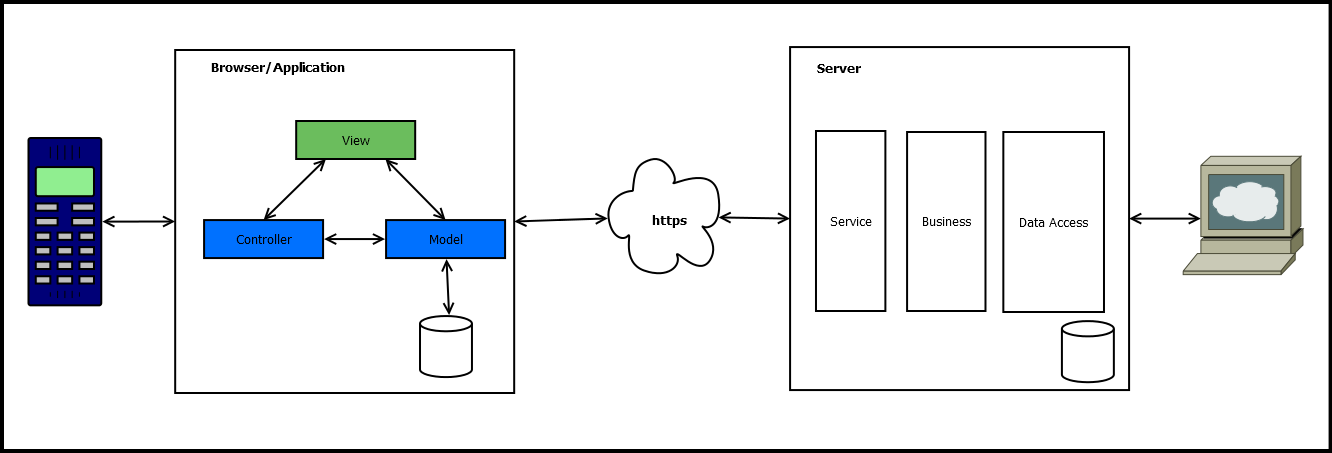
\includegraphics[width=5.5in]{ch4/SOA/SOAArchitecture}
  \caption{SOA Architecture of Smart Cafeteria}
  \label{SOAArchitecture}
\end{figure}


\section{Prototype of Smart Cafeteria}
\label{sec:PrototypeSC}
Prototyping~\cite{Mads2010,Greenberg}, the process of developing prototypes, is
a method used by designers to get feedback from users about future designs.
Prototypes are experimental and incomplete designs of system which are cheap;
can be developed quickly and it is an essential part of iterative user-centered
design.

The main purpose of prototyping is to involve the users in testing design ideas
and get their feedback in the early stage of development, to reduce cost and
save time. It provides an efficient and effective way to optimize interfaces
through interactive discussion and testing. The prototypes can be changed
multiple time until a stable version of user interface that has been
accomplished with efforts both from designers and users.

Prototyping can be divided into three categories; low-fidelity prototyping,
medium-fidelity prototyping and high-fidelity prototyping. In some literature,
it is simply classified as low-fidelity prototyping and high-fidelity
prototyping, where low-fidelity prototyping is mainly about paper-based mock-up
such as Sketches, Storyboard and high-fidelity is mainly about computer-based
simulation. High-fidelity prototypes are fully interactive, simulating most of
the functionality of the final product whereas medium-fidelity prototypes are
computer-based simulation too but it simulates the system interaction and
functionality partially; not all features of the intended system.


I have designed and demonstrate most of the functionalities and requirements
which I have gathered in previous chapter~\ref{chap:AnalysisofSmartCafeteria}.
According to structural diagram (Class Diagram \ref{subsec:classdiagram}) and
dynamic diagram (Activity Diagram \ref{subsec:activity}) in UML 2, I have come
to a stage from where I have proposed a medium fidelity prototype which meets
and shows initial visualization of most fundamental functionalities and
requirements.

To demonstrate and discuss full design template, I will discuss some
functionalities in desktop prototype section \ref{subsec:prototypefordesktop}
and rest of them will be discussed in mobile prototype section
\ref{subsec:PrototypeforMobile}.

\subsection{Desktop Prototype}
\label{subsec:prototypefordesktop}
In this thesis work, I have designed a medium fidelity prototype of smart
cafeteria.


The prototype of smart cafeteria has been designed by
HTML5\footnote{\href{http://www.w3.org/TR/html51/}{HTML 5}},
CSS3\footnote{\href{http://www.w3.org/TR/CSS/}{Cascading Style Sheets (CSS3)}}
and Twitter
Bootstrap\footnote{\href{http://twitter.github.io/bootstrap/}{Twitter
Bootstrap}} jQuery plugins.  To design the template, I have used Eclipse IDE
Juno\footnote{\href{http://twitter.github.io/bootstrap/}{Eclipse IDE}} and run
that on Apache Tomcat server
v7.0\footnote{\href{http://tomcat.apache.org/}{Apache Tomcat server v7.0}}.


There are two basic main part in the prototype; index \ref{indexpage} which will
come after starting the application or browsing the application and dashboard
\ref{dashboardpage} will be accessible after user logs into the system.

\subsubsection{Index}
\label{indexpage}
In the index page, there are a couple of functionalities; among them search food
menu, signup, login, todays hot food menu slider and today's all food menus are
most common. Using user information such as user name and password, user could
go into user dashboard page. There are two steps in signup activity; the first
step is for basic information of user and the last step will ask user's
additional information which will help to calculate user's dieting information
and suggesting food menu by some adaptive mechanism such as machine learning
methods. The functionality of user's password recovery also exists there. There
exists two navigation shortcuts link such as search more menu and time schedule
of cafeteria and branches. This page also contains a list of today's food menu
supported by pagination functionality that are divided into three subcategory;
full menu, half menu and snacks. In full menu, there are three types of menu
courses such as first course (pasta or rice and sauce), second course (fish or
meat and vegetable soup) and desert. Since the proposed system would support as
dynamic content management so we should not concentrate about number of foods
and food menus. In the figure \ref{PLindex}, demonstrate a medium fidelity
prototype of index page of Smart cafeteria system.

\begin{figure}[h!t]
    \centering
    \fbox{
      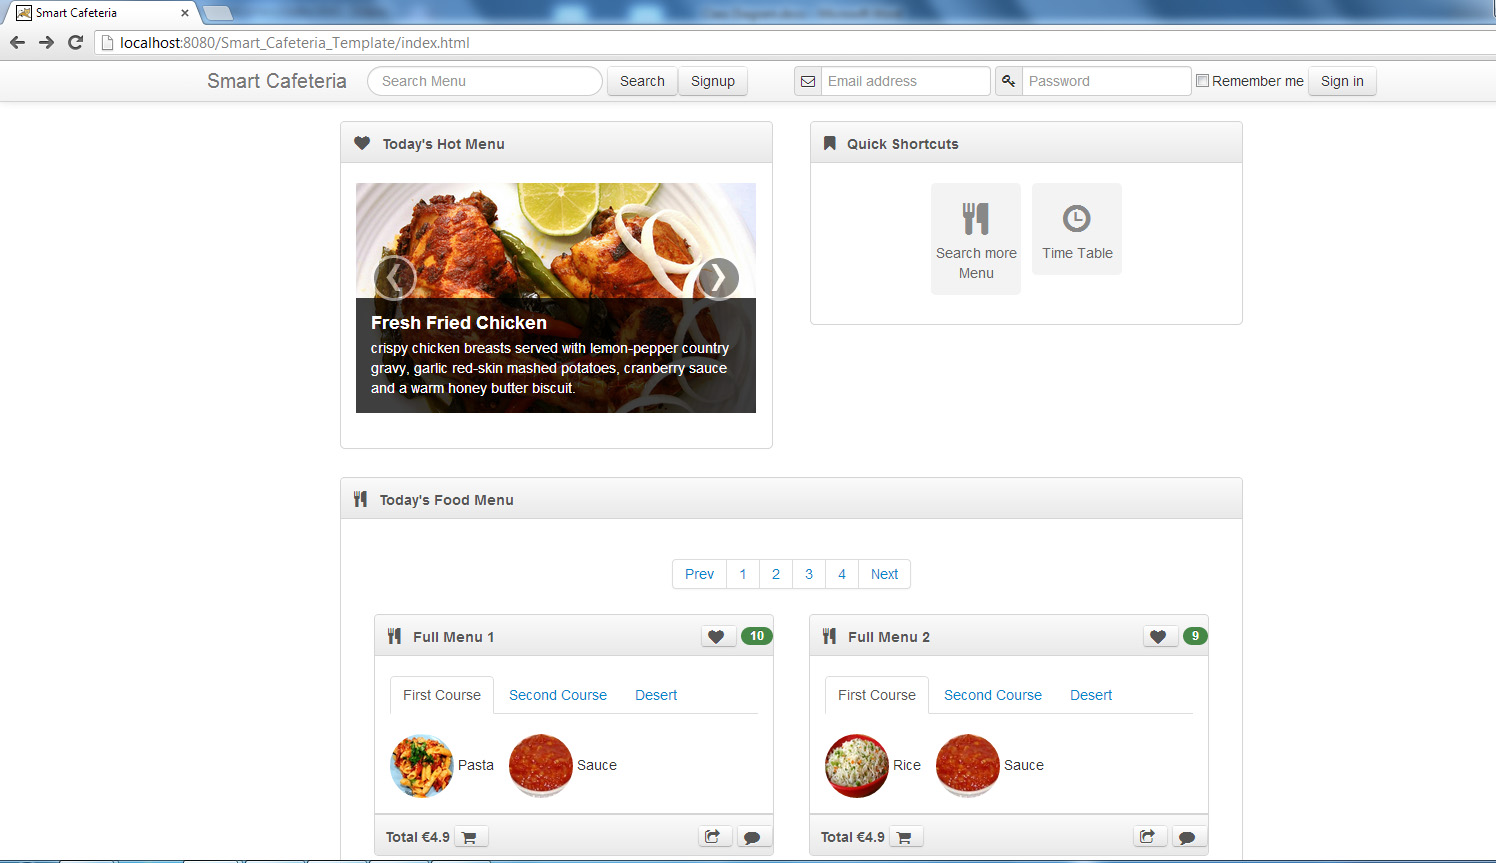
\includegraphics[width=5.5in]{ch4/Prototype/Laptop/index}
      }
  \caption{Index of Smart Cafeteria}
  \label{PLindex}
\end{figure}

\subsubsection{Dashboard}
\label{dashboardpage}
 This is the most important page in the system where credentials are required to
 get access. In this page, there are two sides; upper side of the page
 [Figure~\ref{PLdashboard}] consist navigation shortcuts and a short report of
  food consumption by user and lower side of the page
  [Figure~\ref{PLfoodmenusuggestion}] consists
 suggested food menu by the system using adaptive mechanism (Machine learning
 approach). The navigation shortcuts [Figure~\ref{PLdashboard}] consists
 different functionalities such as search menu, search friends, see follower,
 friend's activities, show dieting reports, create custom menu, show time table
 and branches.
 
\begin{figure}[h!t]
    \centering
      \fbox{
      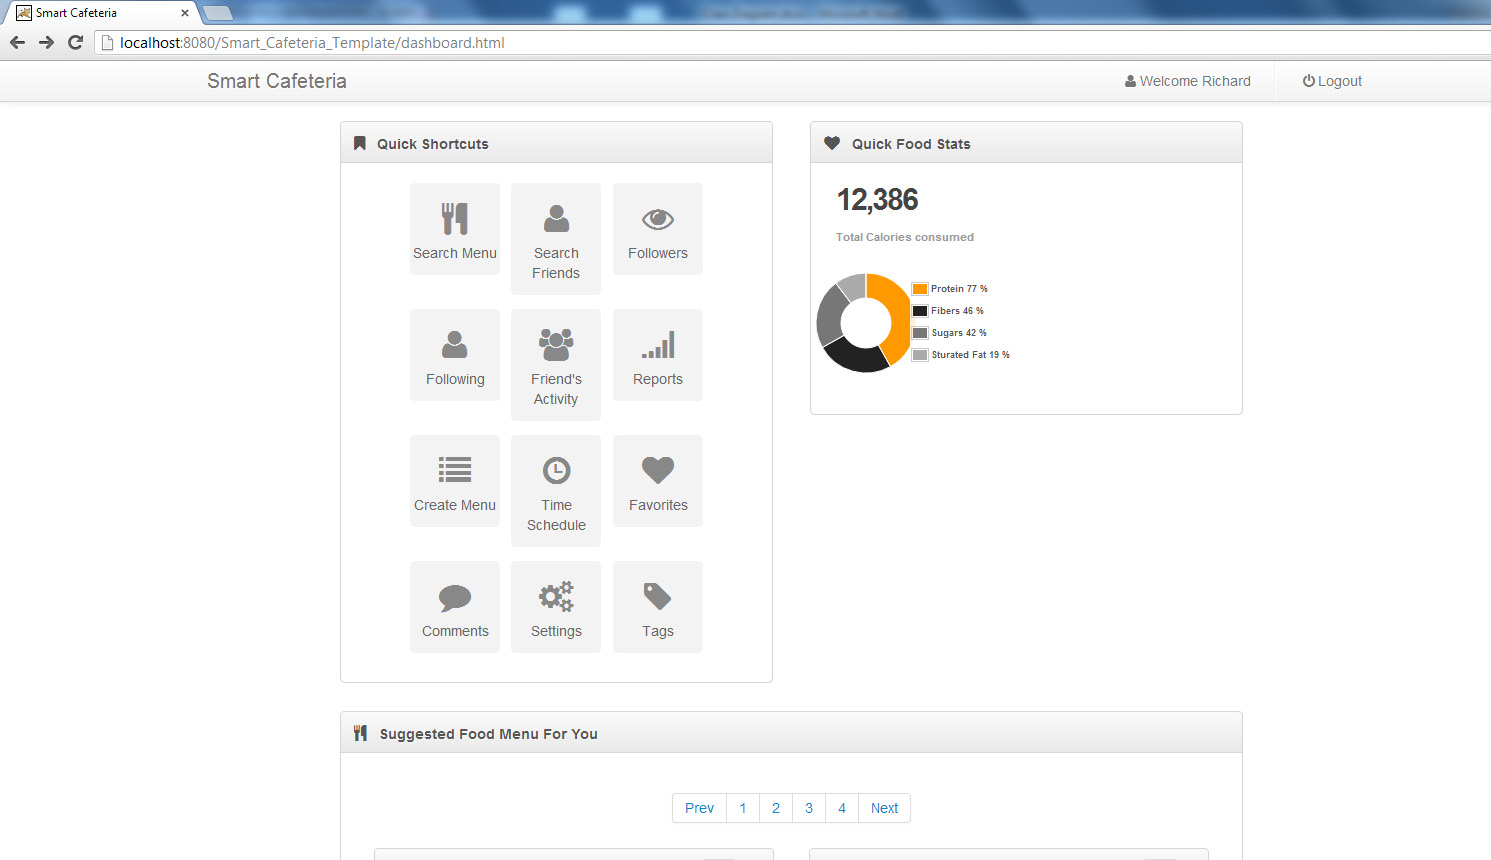
\includegraphics[width=5.5in,height=3.4in]{ch4/Prototype/Laptop/dashboard}
      }
  \caption{Dashboard of Smart Cafeteria [Navigation]}
  \label{PLdashboard}
\end{figure}

\begin{figure}[h!t]
    \centering
      \fbox{
      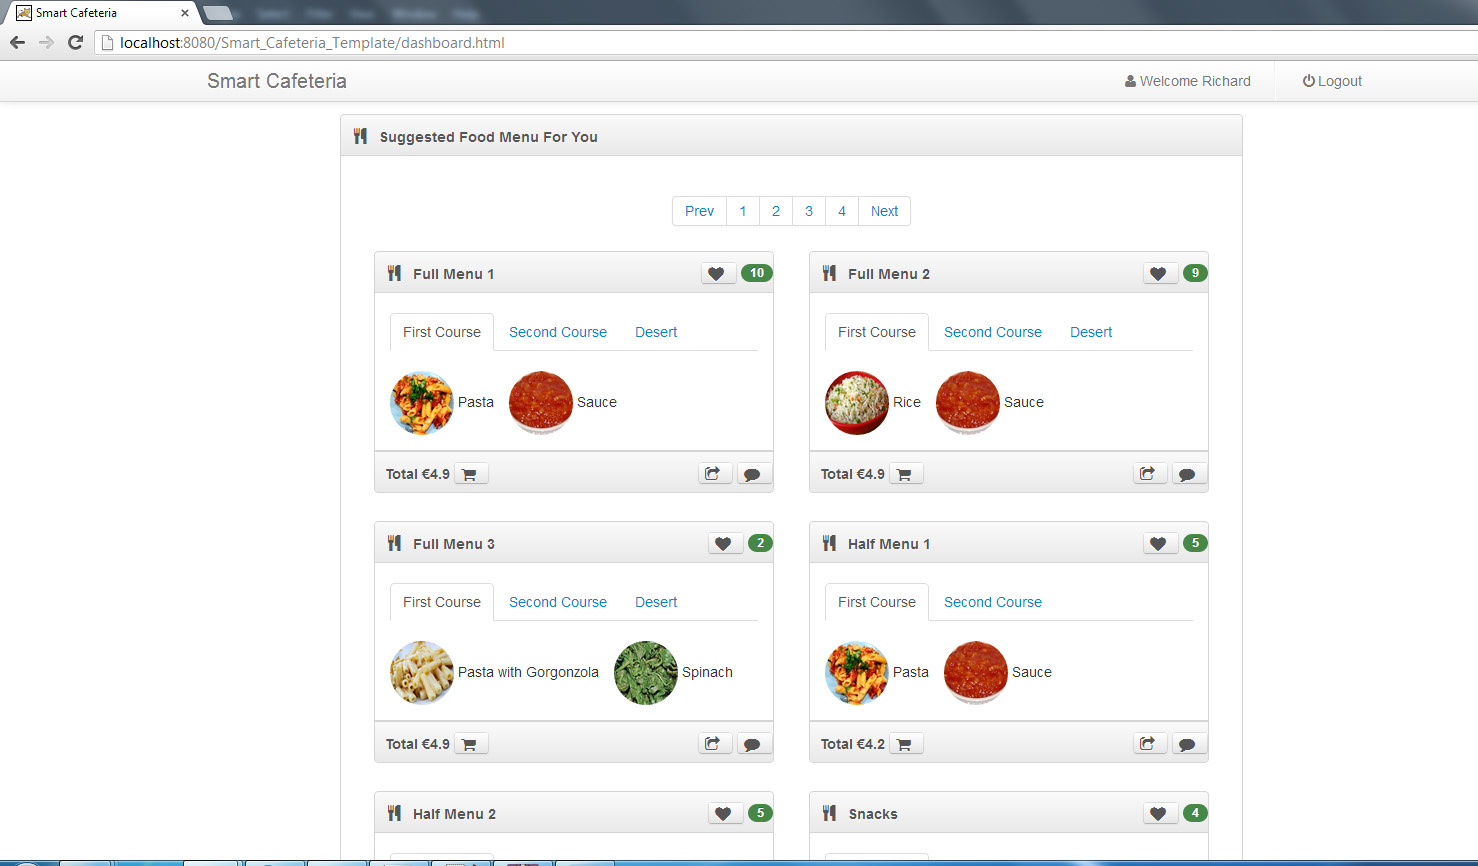
\includegraphics[width=5.5in,,height=3.4in]{ch4/Prototype/Laptop/foodmenusuggestion}
      }
  \caption{Dashboard of Smart Cafeteria [Today's \& Suggested food menu]}
  \label{PLfoodmenusuggestion}
\end{figure}

\newpage
\subsection{Mobile Prototype}
\label{subsec:PrototypeforMobile}
The prototype of smart cafeteria for mobile plateform was designed with HTML5,
CSS3 and Twitter Bootstrap jQuery plugins. To design and demonstrate the
template, I have used phonegap\footnote{\href{http://phonegap.com/}{Phonegap}}
tools for implemention as it supports most of mobile OS such as android, iOS.
I have described some functionalities in the previous
section~\ref{subsec:prototypefordesktop} and the rest of the functionalities of
smart cafeteria I will be demonstrated in this section.

\subsubsection{Index}
\label{Indexpagemobile}
The index page contains search food menu, signup, login, today's hot food menu
slider and today's all food menus offered by cafeteria. In the
figure~\ref{fig:PMInstalledIndex}, left shows installed smart cafeteria apps and
the right shows index page of smart cafeteria.

\begin{figure}[h]
\centering
      \fbox{
\begin{subfigure}[b]{.5\textwidth}
  \centering
    \fbox{
  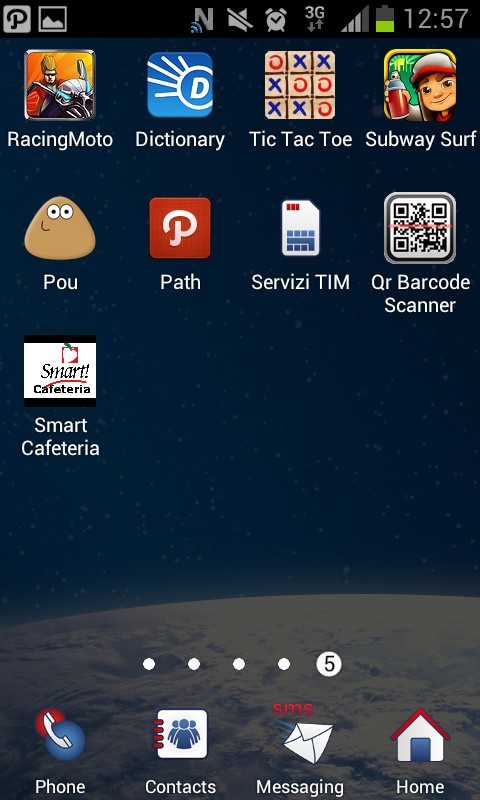
\includegraphics[width=0.9\textwidth]{ch4/Prototype/Mobile/mobile-installed.png}
  }
\end{subfigure}%
\begin{subfigure}[b]{.5\textwidth}
  \centering
  \fbox{
  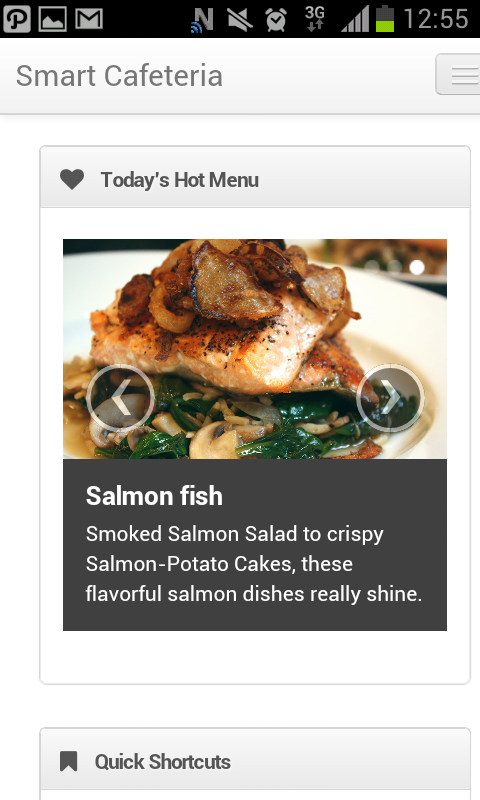
\includegraphics[width=0.9\linewidth]{ch4/Prototype/Mobile/mobile-index.png}
  }
\end{subfigure}
}
\caption{Installed Smart Cafeteria Apps(Left). Index page of Smart Cafeteria (Right).}
\label{fig:PMInstalledIndex}
\end{figure}
\newpage

\subsubsection{User Registration}
\label{UserRegistration}
The registration has two steps; step one needs the basic information of users
such as User Name, Email, password which is shown in left of the figure
\ref{fig:PMUserRegistration} and on the right of the figure
\ref{fig:PMUserRegistration} step two which asks users' physical
information which will help to calculate dieting report and suggest appropriate
food menu is shown.
\begin{figure}[h]
\centering
  \fbox{
\begin{subfigure}[b]{.5\textwidth}
  \centering
   \fbox{
  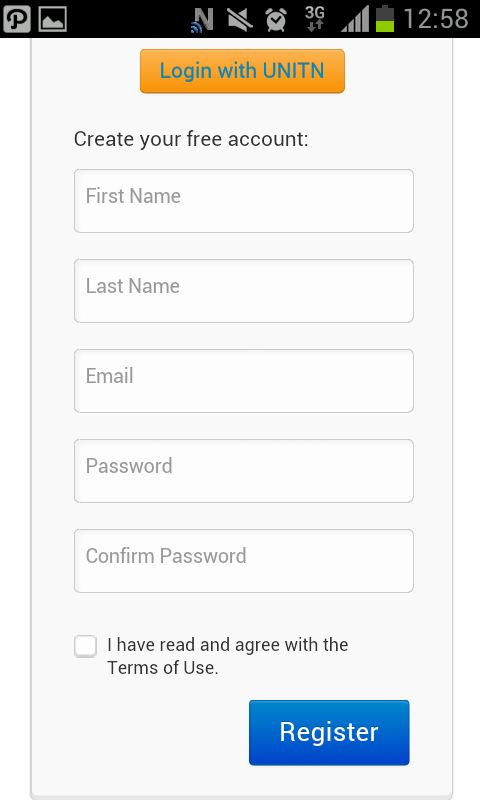
\includegraphics[width=0.9\textwidth]{ch4/Prototype/Mobile/mobile-registration-step1}
  }
\end{subfigure}%
\begin{subfigure}[b]{.5\textwidth}
  \centering
   \fbox{
  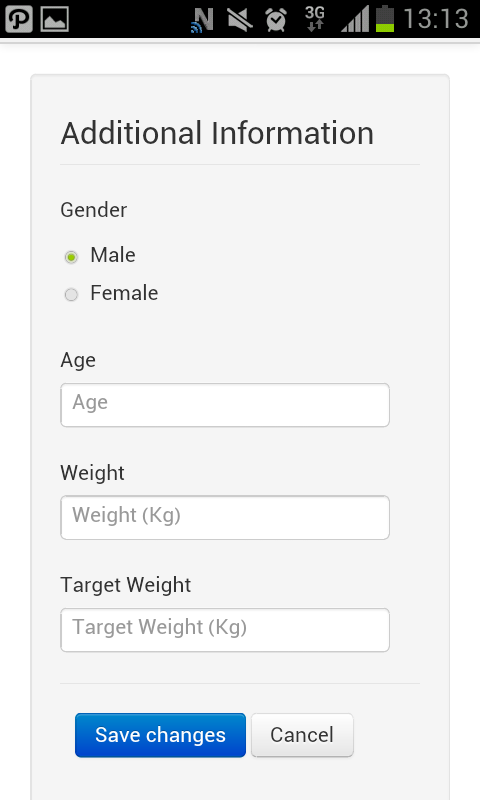
\includegraphics[width=0.9\linewidth]{ch4/Prototype/Mobile/mobile-registration-step2}
  }
\end{subfigure}
}
\caption{User Registration step one of smart cafeteria (Left). User Registration step two of smart cafeteria (Right).}
\label{fig:PMUserRegistration}
\end{figure}


\subsubsection{User Login and Password Recovery}
\label{UserLoginandPasswordRecovery}
To use full functionalities of the system such as order food menu, follow
friends, share lunch item with friends; it is very important to login into the
system. Since sometimes it is essential to recover password in any system,
password recovery also an important function in the smart cafeteria. In the left
of the figure~\ref{fig:PMUserLogin} shows user Login of smart cafeteria and in
the right of the figure~\ref{fig:PMUserLogin} shows user Password Recovery of
smart cafeteria.

\begin{figure}[h]
\centering
  \fbox{
\begin{subfigure}[b]{.5\textwidth}
  \centering
        \fbox{
  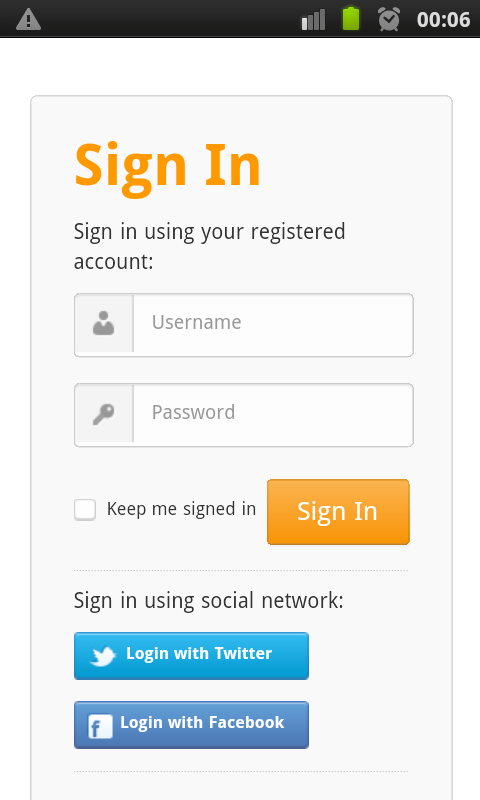
\includegraphics[width=0.9\textwidth]{ch4/Prototype/Mobile/login}
  }
\end{subfigure}%
\begin{subfigure}[b]{.5\textwidth}
  \centering
        \fbox{
  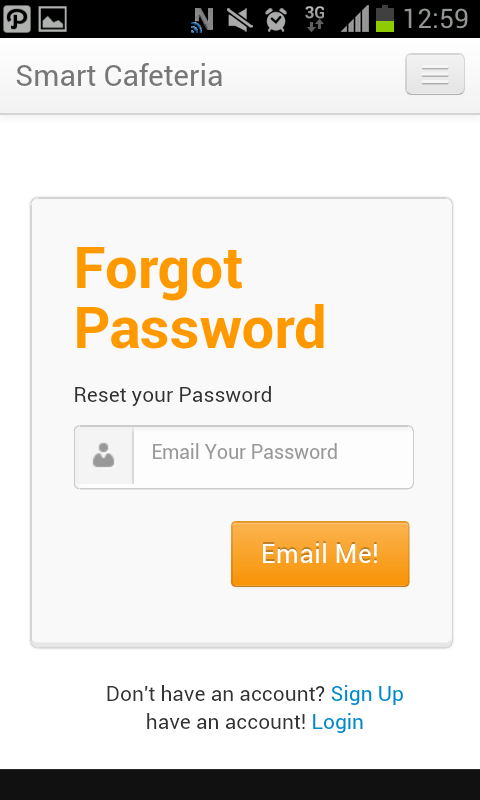
\includegraphics[width=0.9\linewidth]{ch4/Prototype/Mobile/forgotpassword}
  }
\end{subfigure}
}
\caption{User Login of smart cafeteria (Left). User Password Recovery of smart cafeteria (Right).}
\label{fig:PMUserLogin}
\end{figure}

\subsubsection{Generate dieting report}
\label{Generatedietingreport}
Since the system will store the basic information of users as well as their
physical information; using these information through some machine learning
approach, system will generate dieting report, menu suggestion as an adaptive
system. In the left of the figure~\ref{fig:PMReport} shows users dieting report
of smart cafeteria and in the right of the figure~\ref{fig:PMReport} shows
Nutrition Suggestion for user of smart cafeteria.

\begin{figure}[h]
\centering
      \fbox{
\begin{subfigure}[b]{.5\textwidth}
  \centering
        \fbox{
  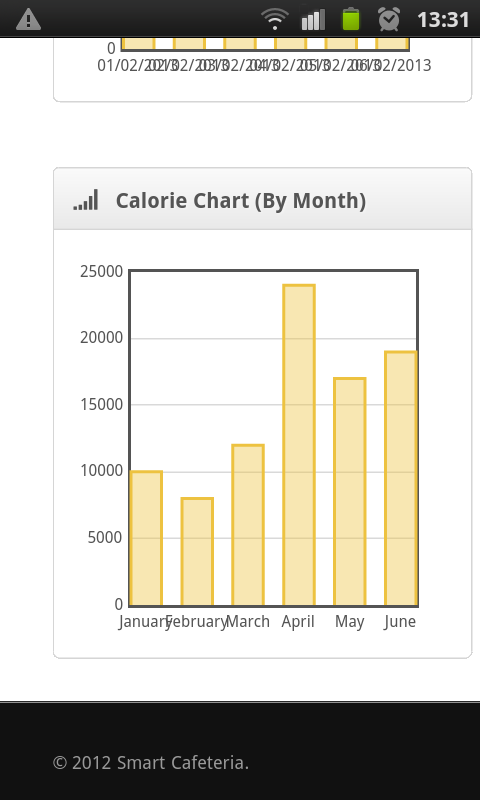
\includegraphics[width=0.9\textwidth]{ch4/Prototype/Mobile/report}
  }
\end{subfigure}%
\begin{subfigure}[b]{.5\textwidth}
  \centering
        \fbox{
  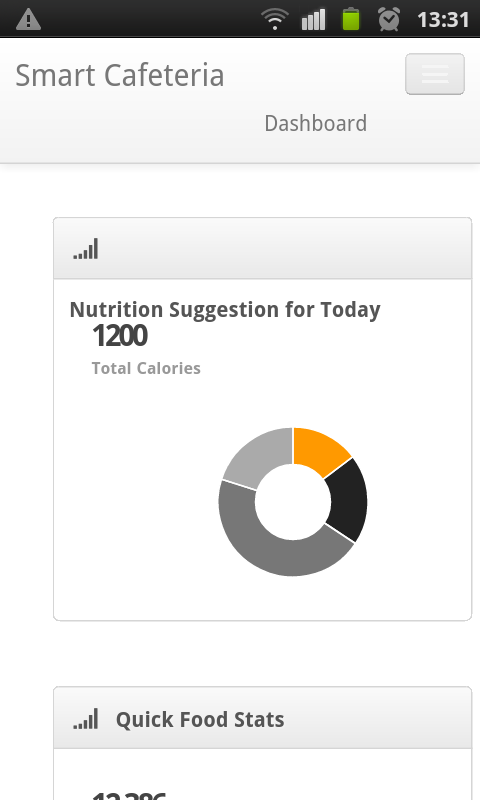
\includegraphics[width=0.9\linewidth]{ch4/Prototype/Mobile/suggestion}
  }
\end{subfigure}
}
\caption{Dieting Report for User of smart cafeteria (Left). Nutrition Suggestion of smart cafeteria (Right).}
\label{fig:PMReport}
\end{figure}
\newpage

\subsubsection{Collaborative and Sharing Activities}
\label{Searchfollowingfriends}
Since Smart cafeteria support collaborative activities, the design template
consists those functionalities: search friends, follow friends and sharing their
activities which will make the system more interactive and usable in user
prospective. In the left of the figure~\ref{fig:PMUserFollow} shows following
friends functionality of smart cafeteria and in the right of the
figure~\ref{fig:PMUserFollow} shows friends activity of smart cafeteria.

\begin{figure}[h]
\centering
      \fbox{
\begin{subfigure}[b]{.5\textwidth}
  \centering
        \fbox{
  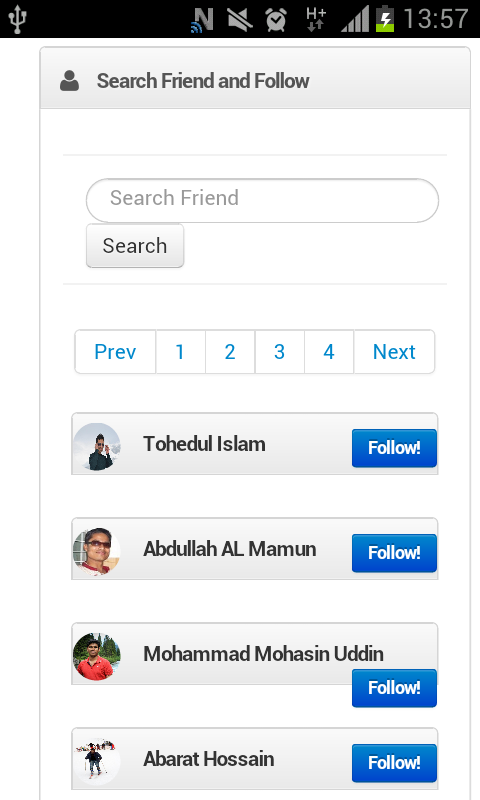
\includegraphics[width=0.9\textwidth]{ch4/Prototype/Mobile/following}
  }
\end{subfigure}%
\begin{subfigure}[b]{.5\textwidth}
  \centering
        \fbox{
  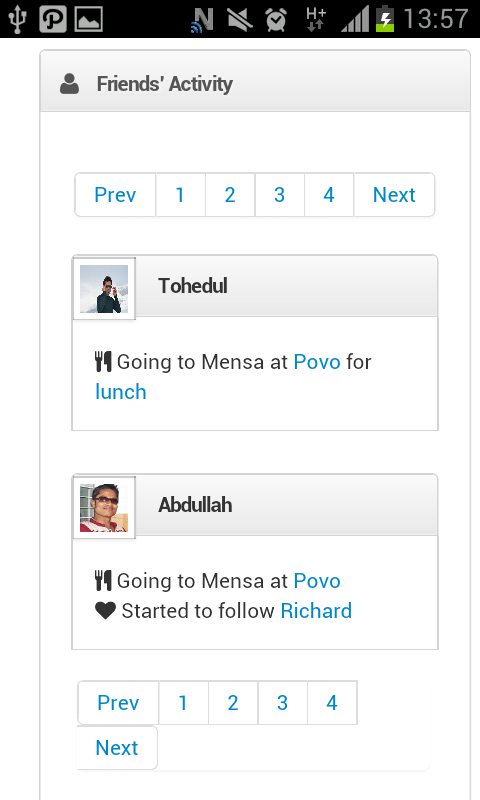
\includegraphics[width=0.9\linewidth]{ch4/Prototype/Mobile/friendsactivity}
  }
\end{subfigure}
}
\caption{: Following Friends for User of smart cafeteria (Left). Friends activity of smart cafeteria (Right).}
\label{fig:PMUserFollow}
\end{figure}
\newpage

\section{Key Features of Smart Cafeteria}
\label{sec:keyFeaturesSC}
There are three key feature in proposed smart cafeteria system which will
support this system's analysis as a research work. The features are listed and
describing bellow:

\subsection{Online Cafeteria services}
The application will provide online cafeteria services where user could search
food menu, order online food menu, pay online that will support
university's cafeteria queue skipper; namely users could browse and choose their
food menu before entering cafeteria. Thus user could easily skip long queue that
seems to be very annoying task in every day lunch time at university. At the same
time, through this application, user could get knowledge about every day food
menu in different branch and acknowledge about time schedule of all branches of
cafeteria. This is very important services now days in university to make life
easy and enjoyable.

\subsection{Adaptive services}
The application will provide online adaptability services such as daily menu
suggestion based on users' previous choice and calorie consumption of the users
in the last couple of weeks. The system will also provide dieting report of
every user which makes the life of the people more comfortable, more enjoyable
and happier. This is very important issue especially for students so these
adaptive services will have a great significance in university life without any
doubt.

\subsection{Social collaboration services}
The application will provide such an environment where user could interact in
social collaboration such as follow friends, share food menu with friends, share
activities of social eating as well as can see friend's activities. These services
will help students to increase collaboration between domestic students with
international students due to exchange food culture, language or psychological
peer supporting.

\subsection{Mobile Interaction}
Now a days, only web 2.0 applications are not sufficient to provide services to
users; a huge number of users want to get the application's services using Smart
phone. People are now used to get portable services to ensure maximum level of
satisfaction and enjoyable experience from application. Since Smart cafeteria
will provide services to university students, so all services and
functionalities of Smart Cafeteria should be supported by mobile apps and tablet
apps. So the plan is to make the application services portable, enjoyable,
usable using smart phone application  to help students.

